\documentclass[
fontsize=10pt,
font-family=lmodern,
languages={british,french}, % 'british' ou 'american' (pas 'english' !)
main-language=french,
load-style=dg,
title-font-family=sans-serif,
header-style=chapter-section,
bibliography-style=dg,
]{mines-albi-these}

% les glossaires (index et nomenclature)
\makeglossaries
% ------------------------------------------------------------
% déclaration des acronymes (pour l'index)
% ------------------------------------------------------------

\newacronym{IMT}{IMT}{Institut Mines-Télécom : depuis 2017, intégration
  dans un seul institut des écoles de télécom et de la plupart des
  écoles des mines, sous la tutelle du ministère de l’Économie et des
  Finances.}

%%% Local Variables:
%%% mode: latex
%%% TeX-master: "../ma-these"
%%% End:

% ------------------------------------------------------------
% déclaration des symboles (pour la nomenclature)
% ------------------------------------------------------------

\newsymbolentry{sigma}{
  type=greek letter,
  sort={sigma},
  name={$\sigma$},
  description={Tension superficielle},
  unit={\si{\N\per\m}},
}

\newsymbolentry{Scap}{
  type=alphanumeric,
  sort={Scap},
  name={\ensuremath{S_{cap}}},
  description={Surface de la section du capillaire},
  unit={\si{\square\m}},
}

%%% Local Variables:
%%% mode: latex
%%% TeX-master: "../ma-these"
%%% End:


% pour la couverture
\usepackage{mines-albi-these-frontpage}

% une source de références bibliographiques
\addbibresource{bibliographie/ma-biblio.bib}

% la méta-information (dans le PDF et éventuellement sur la couverture)
\author{Prénom Nom}
\title{Un titre très long qui donne envie de lire toute la thèse}
\date{1\up{er} décembre 2099} % date prévue de soutenance

\begin{document}

%----------------------------------------
\frontmatter


\makefrontpage{
  %% ----------------------------------------
  %% bandeau (à supprimer en version finale
  label=Review version,
  %% ----------------------------------------
  %% thèse délivrée par
  granted by=imt mines albi,
  %% ----------------------------------------
  %% unité de recherche (utilisée les valeurs prédéfinies si possible)
  new research unit={mon labo}{CGI -- Centre Génie Industriel, IMT Mines Albi},
  research unit=mon labo,
  %% ----------------------------------------
  %% école doctorale (utilisée les valeurs prédéfinies si possible)
  new phd school={ednew}{EDSYS : Informatique et Génie Industriel},
  phd school=ednew,
  %% ----------------------------------------
  %% l'auteur (à décommenter si différent de la méta-information)
  % full name={Prénom Nom},
  %% ----------------------------------------
  %% la date de soutenance prévue (à décommenter si différent de la méta-information)
  % date={1\up{er} décembre 2099},
  %% ----------------------------------------
  %% le titre (à décommenter si différent de la méta-information)
  % title={Un titre très long qui donne envie de lire toute la thèse},
  %%  ----------------------------------------
  %% la (co)direction de thèse
  %% Le directeur apparait en premier 
  supervision labels={Directeurs de thèse :}, % {singulier}{pluriel}
  supervisor/.list={
      {Prénom Nom, Professeur, Mines Albi, \small{Albi}},
      {Prénom Nom, Professeur, Université XXXX, \small{Xxxx}}
    },
  %% ----------------------------------------  
  %% les membres du jury (le président n'est connu qu'après la soutenance) sans la direction
  %% Si rapporteur absent - mentionné sur la page de titre (pas pr examinateur)
  jury/.list={
      {M\up{me} Prénom Nom, Professeur, Université du XXXX, \small{XXXX} \textit{(Président)}},
      {M. Prénom Nom, Professeur, Université du XXXX, \small{XXXX} \textit{(Rapporteur)}},
      {M. Prénom Nom, Professeur, Université du Temps Libre, \small{XXXX} \textit{(Rapporteur)}},
      {M\up{lle} Prénom Nom, Maître assistant, Mines Albi, \small{Albi} \textit{(Examinateur)}},
      {M. Prénom Nom, Maître assistant, Mines Albi, \small{Albi} \textit{(Invité)}}
    },
}

%%% Local Variables:
%%% mode: latex
%%% TeX-master: "../ma-these"
%%% End:


\summary

\chapter*{Remerciements}

Cette partie est le point final de ces travaux et s'avère également être la dernière page de ce chapitre personnel.
Comme toutes les bonnes aventures, elle n'aurait bien sûr pas été aussi plaisante sans de nombreux compagnons.
Je ne remercierai jamais assez chacun d'eux.

Tout d'abord, mon encadrement de thèse, et en particulier mon directeur et ma directrice.
Frédérick, pour son enthousiame permanent et son incroyable ambition pour ce que je créais.
Nos conversation ont été nombreuses et pourtant j'ai le sentiment qu'il n'y en a pas eu assez,
tant elles ont été productive intellectuellement.
Je peux heureusement me consoler en sachant qu'il y en aura d'autres.\\
Andrea qui a apporté une couleur toute personnelle à ces travaux.
Tout d'abord par son accueil chaleureux lors de mon temps aux États-Unis, ce qui m'a permit d'aborder ces travaux avec un autre regard.
Il va sans dire que ses contributions ne s'arrêtent pas là.
Elle a été un inestimable soutient me supporter et m'accompagner dans mes raisonnements tout au long de ce projet, et pour cela je lui suis très reconnaissant.
J'espère qu'un jour nos chemins se recroiseront de nouveau.

Bien évidemment vient ensuite Aurélie, qui a su marquer ces travaux par son intelligence
mais aussi sa bienveillance et son attention. Tu as su être disponible quand j'avais besoin
de toi et m'aider dans les moments les plus difficiles, et pour cela, je te suis incroyablement reconnaissant.
Tout comme pour Fred, nos innombrables (et parfois longues) conversations qui ont su alimenter nos réflexions respectives.
J'espère que l'on trouvera du temps pour en avoir d'autres.

Je tiens également à remercier Tina Comes et Valentina Dragos d'avoir accepté de relire en détail le présent manuscrit.
Je dois reconnaître leurs patience pour affronter autant de contenu aussi rigoureusement, et les remercier pour leurs nombreuses commentaires perspicaces qui ont su améliorer substantiellement ce manuscrit.

Je remercie également François Charoy, d'avoir habillement présidé le jury de ma soutenance et pour ses remarques profondes sur mes travaux.

En tant qu'invités, j'ai bien évidemment été ravi de revoir Prasenjit Mitra et Jess Kropczynski à cette occasion, en gage de leurs bienveillance sur mes travaux lors de mon passage aux États-Unis.

Caroline Rizza, pour sa gestion du projet MACIV, ainsi que tous les autres acteurs du projet, qui ont permis les nombreuses rencontres et les nombreux retours dont ce travail à amplement bénéficié.

Parmi tous mes compagnons dans cette aventure, certains ont su faire de ce long voyage, un voyage moins long.
Oversea, I obviously think about my housemates, Chloe, Laura and Adam, Erinn, Ryan but also Jenny, Nasim, Connor and Guillermo.
It was good having you around and I definitely miss spending time with you around State College.

- Audrey et Guillaume
- Aurelie et Robin
- Eva
- Raphael
- Robin
- Manon
- Sina

Vous avez définitivement donné une teinte bien plus colorée à cette expérience, au rythme
des nombreuses session de jeux et des nombreux autres moments que l'on a pu échanger ensemble.
Les nombreux moments que l'on a passé ensemble (café etc.)

Mes parents, ma sœur et ma famille en general qui m'ont supporte et encouragé tout au
long de ce voyage vers ces contrés bien lointaines.
Cette réussite .

%%% Local Variables:
%%% mode: latex
%%% TeX-master: "../ma-these"
%%% End:


%----------------------------------------
\mainmatter

\chapter*{Introduction}
At the time of writing, humanity is in the second year of the COVID-19 pandemic, at the dawn of the Omicron variant.
In its propagation, this virus has led the world in a crisis of a magnitude usually contained in History books.
All the world countries are currently facing a multifaceted crisis involving public health, social and economic issues.
However, suppose we detach ourselves from the current events.
In that case, we realize two points: (i) that crises and society are historically two partners in the same dance, and (ii) that despite the prevailing fear and uncertainty, society is still very much present.
In the heat of the moment, it is difficult to perceive our societies' extraordinary resilience, regardless of the times.
This resilience is made possible by the individuals of the society who manage this crisis, each at their own level.

This event reminds everyone of the importance and difficulty of crisis management.
Crisis management is, above all, a matter of making decisions with uncertain information and an uncertain environment.
In this context, facilitating access to and processing of information becomes key issue.
At the same time, accessing and processing information has never been easy.
The democratization of social media and the development of Artificial Intelligence methods have allowed significant progress on these aspects.

\emph{How to automatically leverage information posted on social media during a crisis?}
From this interrogation, three scientific questions are extracted:

\begin{enumerate}
    \item What information posted on social media is helpful for crisis response?
    \item How can we automatically collect this information?
    \item How to effectively deliver this information to the decision-makers in charge of the response?
\end{enumerate}

These questions were explored during the ANR MACIV project (Management of Citizens and Volunteers: the social media contribution in crises).
This project brought together different actors, both institutional (Direction Générale de la Sécurité Civile et de la Gestion des Crises, Préfecture de Police de Paris, Service Départemental d'Incendie et de Secours du Var),
associations (VISOV: Volontaires Internationaux en Soutien Opérationel Virtuel) and academics (Centre Génie Industriel - IMT Mines Albi and Institut Interdisciplinaire de l'Innovation - Télécom Paris).
This work also benefited from a welcome cultural diversity thanks to a one-year exchange in the United States at the College of Information Sciences and Technology of the Pennsylvania State University, which allowed us to observe and understand management issues in a context that is certainly familiar but nevertheless different.
All of these actors have contributed to the reflection and the results of this work.

The latter is organized into five parts.
The Figure~ref{introduction:big-picture} outlines the organization by specifying the origin of the entries that allowed each contribution.
The first two parts provide the reader with an understanding of the context and the issues surrounding the topic discussed.
The following three parts break down the contribution of this dissertation into three parts: (i) characterization of the information need, (ii) automatic collection of this need, and (iii) integration of this collection within an information system.

Chapter 1 presents the general context of crisis management, social media, and automated language processing.
A principal research question and three consecutive research questions are identified from this context.

Chapter 2 is a literature review of the research conducted around each research question in recent years.
This literature review feeds into the reflections conducted in the following three chapters.
Each chapter successively answers the research questions.

Chapter 3 identifies the actionable information available on social media for decision-makers when responding to an event.
This information is then organized into an information model used in the following chapters.

Once information that composes actionable information is identified and organized, Chapter 4 proposes an automatic collection method.
This method relies on a semi-supervised machine learning model identifying previous actionable information in messages posted on social media.
The information present in the messages is then highlighted to facilitate the emergency staff's processing of the data stream.

Finally, Chapter 5 considers the processing of social media by the information system as a whole.
In particular, it highlights the crucial role of the information system in both data and information processing.
It argues that an information system containing machine learning models should be organized with two systems in mind: a data system and an information system.

The Conclusion summarizes the contributions and outlines the perspectives for future work.

\begin{figure}[h]
    \centering
    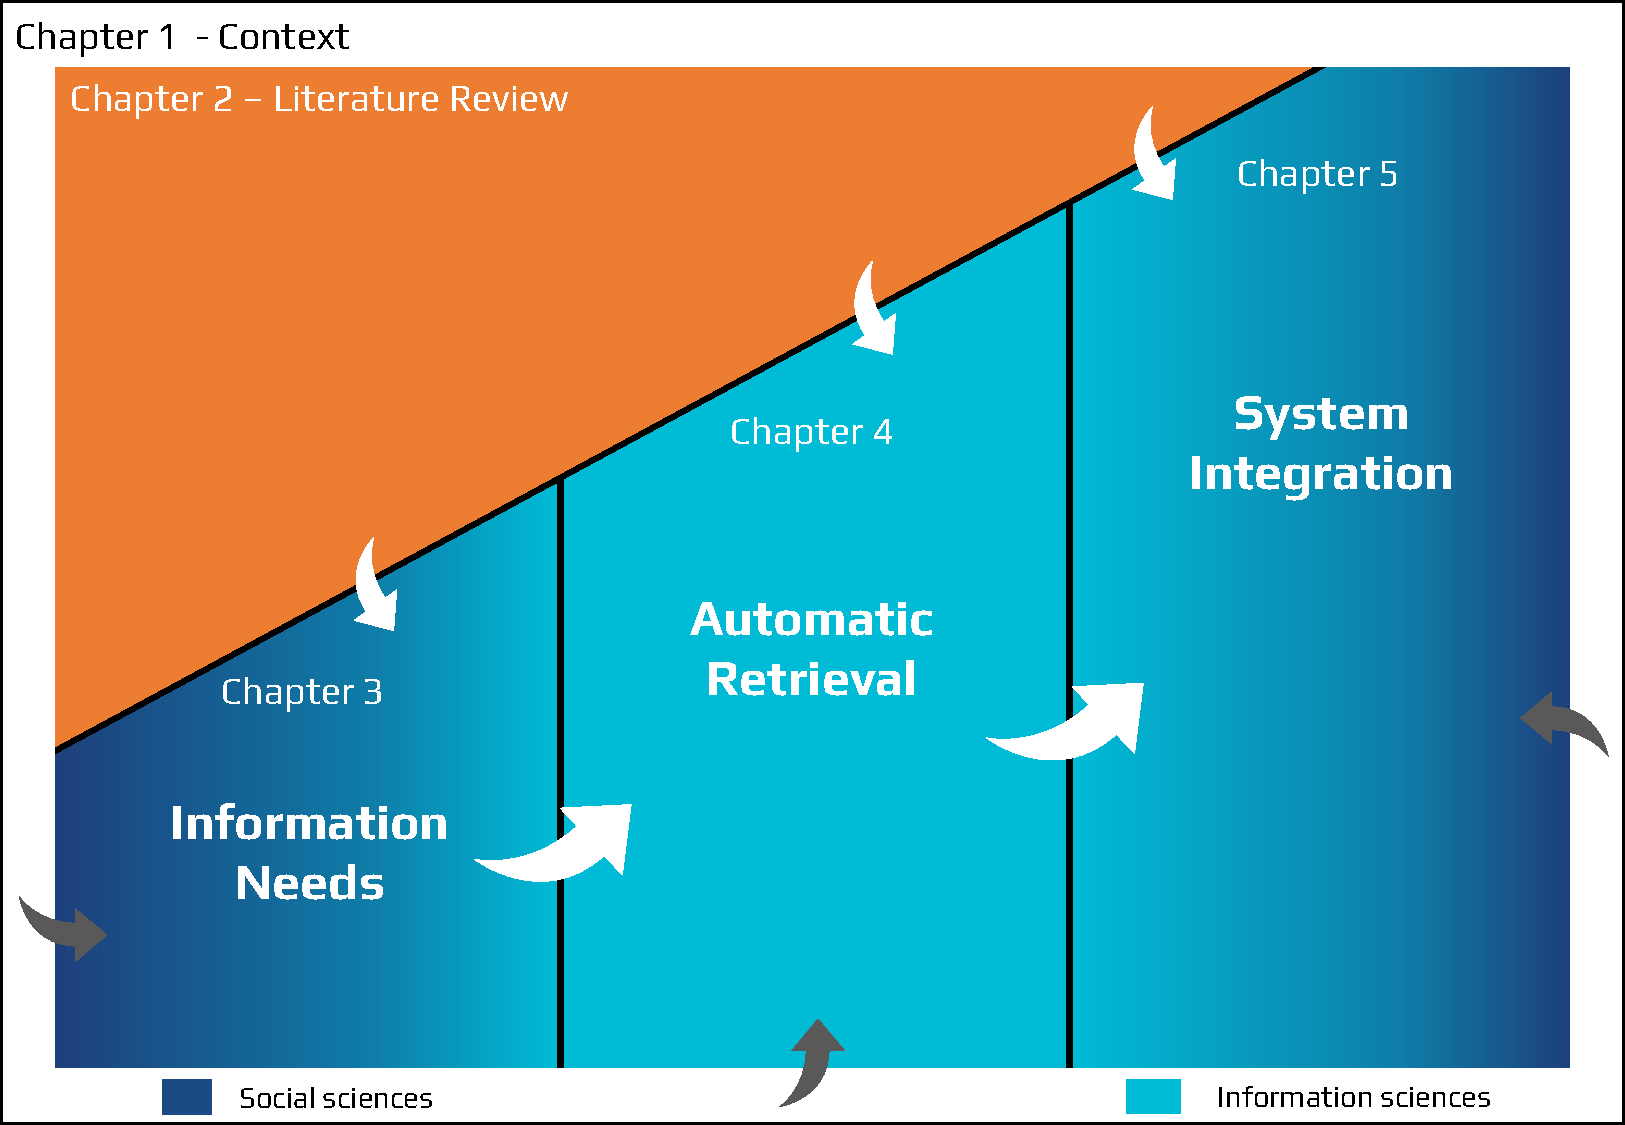
\includegraphics[width=0.92\textwidth,keepaspectratio]{figures/chap-0/big-picture.pdf}
    \caption{Overall organisation of the document. The arrows indicate the contribution of each part on the others.}
    \label{introduction:big-picture}
\end{figure}

%%% Local Variables:
%%% mode: latex
%%% TeX-master: "../ma-these"
%%% End:


\chapter{État de l'art}

Ici, on décrit l'état de l'art...

\begin{table}[bp]
  \centering
  \begin{tabular}{rrr}
    & A & B \\
    \toprule
    Exemple 1 & 10 & 35 \\
    Exemple 2 & 12 & 33 \\
    \bottomrule
  \end{tabular}
  \caption{Un exemple de tableau}
  \label{tab:ex}
\end{table}

%%% Local Variables:
%%% mode: latex
%%% TeX-master: "../ma-these"
%%% End:


\chapter{Problématique}

Ici, on décrit la problématique... Avec la jolie figure \ref{fig:ex}.

\begin{figure}[bp]
  \centering
  
\begin{tikzpicture}
    \fill[orange] circle(1);
    \fill[lime] (1,1) rectangle ++(1,1);
  \end{tikzpicture}
  \caption{Exemple de figure}
  \label{fig:ex}
\end{figure}


%%% Local Variables:
%%% mode: latex
%%% TeX-master: "../ma-these"
%%% End:


\chapter{Ma solution}

Ici, on décrit une solution... En utilisant des acronymes tels que
\gls{IMT}.

%%% Local Variables:
%%% mode: latex
%%% TeX-master: "../ma-these.tex"
%%% End:


\chapter{Expérimentation}

Ici, on décrit l'expérimentation...  Avec utilisation de \gls{sigma} et
de \gls{Scap} !


%%% Local Variables:
%%% mode: latex
%%% TeX-master: "../ma-these"
%%% End:


\chapter*{Conclusion}

La conclusion générale de la thèse...


%%% Local Variables:
%%% mode: latex
%%% TeX-master: "../ma-these"
%%% End:


\appendix

\chapter{Appendix A}

\begin{landscape}
    \begin{figure}
        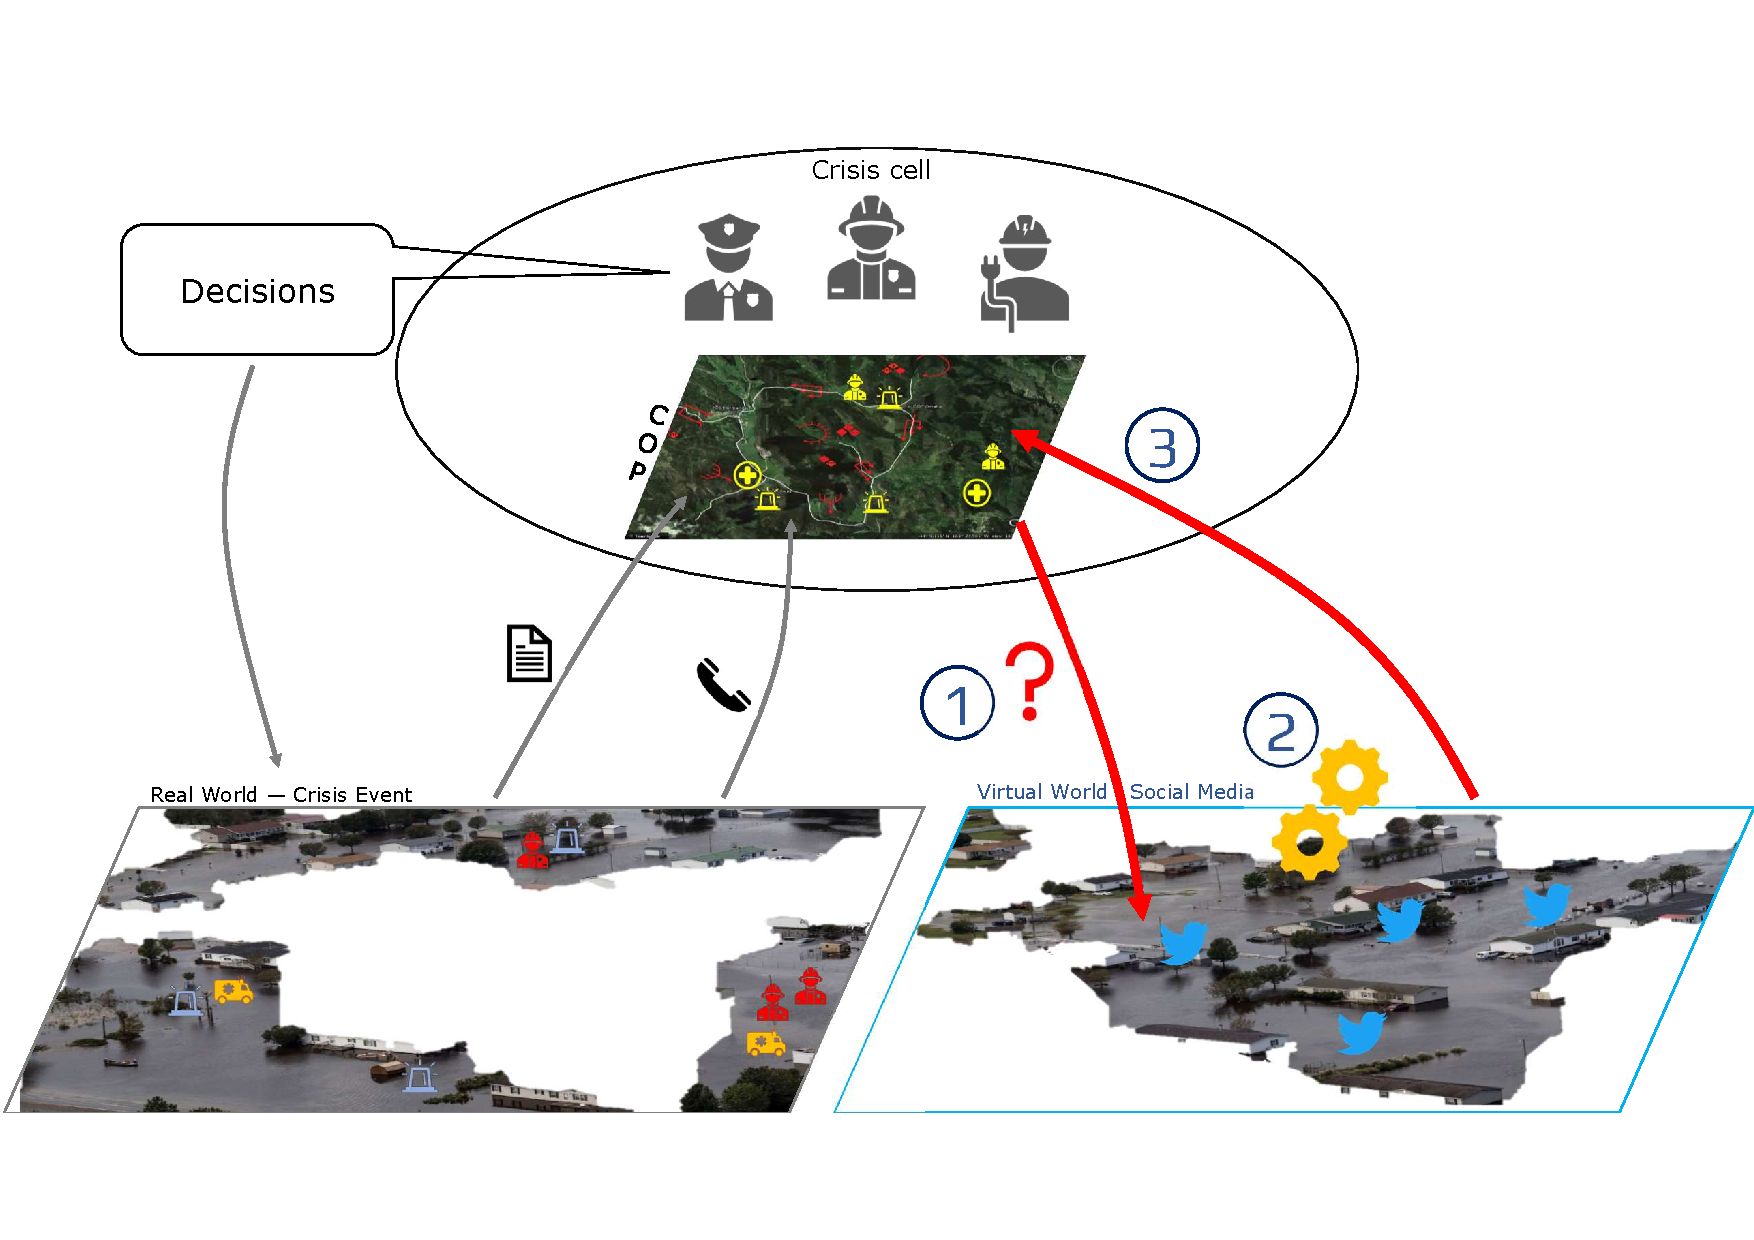
\includegraphics[width=\paperwidth,height=\paperheight,keepaspectratio]{figures/big-picture.pdf}
        \caption{Formal representation of the Information model presented Chapter 3 using the UML 2.0 langage.}
        \label{information:information-models-uml}
    \end{figure}
\end{landscape}

%%% Local Variables:
%%% mode: latex
%%% TeX-master: "../ma-these.tex"
%%% End:


\chapter{Une seconde annexe}

Ici, le contenu de la seconde annexe...

%%% Local Variables:
%%% mode: latex
%%% TeX-master: "../ma-these"
%%% End:


%----------------------------------------
\backmatter

\listoffigures

\listoftables

\listofsymbols % la nomenclature

% Les acronymes
{
  \renewcommand*\glspostdescription{\matmdotfill}
  \printacronyms[style=list,nogroupskip]
}

% la bibliographie
\printbibliography[heading=chapter]

\tableofcontents

% le résumé (en 4e de couverture)
\cleardoublepage
\pagestyle{empty}
\null
\newpage
\abstract[0.6]%
{french}{Résumé}%
{Conception d'un système de traitement des médias sociaux en réponse de crise : extraction, gestion et distribution des informations pertinentes pour les décideurs.}%
{
  Nos sociétés ont toujours été ponctuées de situations de crises, mais la complexité croissante de ces
  événements exige une amélioration constante des méthodologies et des outils employés lors de la réponse.
  L'établissement d'une conscience de la situation commune à tous les acteurs impliqués est l'une de ces améliorations
  potentielles.
  Cependant, cette axe d'amélioration souffre de difficultés liées au manque de ressources à allouer à cette tâche.
  L'automatisation d'une partie des tâches pour supporter le personnel en charge de cet aspect, est donc une opportunité de recherche.
  Cette opportunité est également favorisée par le développement des médias sociaux en tant que sources de données massives.
  Simultanément, le domaine de l'intelligence artificielle a été radicalement modifié par
  le développement de nouveaux outils et de nouvelles méthodes, permettant la recherche
  d'informations complexes au sein de données textuelles.
  À la croisée de ces trois opportunités conjugués, cette thèse explore la question suivante :
  Comment concevoir un système d'information capable de gérer et de fournir automatiquement
  des informations pertinentes extraites des données des médias sociaux ?

  Une approche en trois temps est proposée. Premièrement, il s'agit de comprendre
  quelles sont les informations pertinentes lors de la phase de réponse à une crise pour les preneurs de décision.
  Deuxièmement, une fois les informations pertinentes identifiées, un nouveau module d'intelligence
  artificielle dédié extrait les éléments pertinents à partir des données disponibles sur les médias sociaux.
  Ces informations sont alors intégrées dans un modèle de situation de crise, permettant
  de les organiser automatiquement avec le reste du contexte.
  La troisième et dernière partie discute de l'organisation des données et
  des informations au sein d'un système d'aide à la décision pour la gestion de crise.
  Cette discussion s'intèresse particulièrement à la question de la bonne gestion et de
  la distribution de ces informations auprès des décideurs.
  Cette recherche a été menée dans un contexte international : le projet français ANR
  MACIV, une collaboration entre IMT Mines Albi et Penn State University et en relation
  étroite avec des praticiens français et américains.

  \keywords{Mots-clés :}{Gestion de crise, Apprentissage Machine, Traitement Automatique du Langage, Connaissance de la Situation, Système d'information}
}
{american}{Abstract}%
{Design of a social media processing system for crisis response: extraction, management and delivery of relevant information for decision makers}%
{
  Our societies have always been punctuated by crises, but the increasing complexity of these events requires a constant improvement of the methodologies and tools used in the response.
  Establishing a common situational awareness among all actors involved is one of these potential improvements.
  However, challenges arise due to the lack of available resources to allocate to this task during crisis response.
  The automation of certain tasks to support teams' dedicated actionable information collection, therefore, represents a research opportunity.
  This opportunity is also enabled by the expansion of social media as big data sources.
  At the same time, the field of artificial intelligence has been radically changed by the development of new tools and methods, allowing the retrieval of complex information within textual data.
  At the crossroads of these three opportunities, this dissertation explores the following question:
  How to design an information system capable of managing and automatically providing relevant information extracted from social media data?

  A threefold approach is proposed.
  The first part aims at understanding what information is relevant in the crisis response phase for decision-makers
  Second, once the relevant information is identified, a new, dedicated artificial intelligence
  module extracts the relevant elements from the data available on social media.
  This information is then integrated into a crisis model, allowing to automatically
  pair it with associated information available in the context.
  The third and last part discusses the organization of data and information within a decision support system for crisis management.
  This discussion is particularly interested in designing a system that can achieve proper management and distribution of information to decision-makers.
  This research was conducted in an interdisciplinary context: the French ANR MACIV project, a collaboration
  between IMT Mines Albi and Penn State University and in close relationship with French and American practitioners.

  \keywords{Keywords:}{Crisis Management, Machine Learning, Natural Language Processing, Situation Awareness, Information System}
}

%%% Local Variables:
%%% mode: latex
%%% TeX-master: "../ma-these"
%%% End:


\end{document}

%%% Local Variables:
%%% mode: latex
%%% TeX-master: t
%%% End:
